\documentclass[13pt, a4paper, twoside]{article}
\usepackage[utf8]{inputenc}
\usepackage{geometry}
\usepackage[czech]{babel}
\usepackage{enumitem}
\usepackage{fancyhdr}
\usepackage{amsmath}
\usepackage{mathtools}
\usepackage{float}
\usepackage{setspace}
\usepackage{multicol}
\usepackage{graphicx}
\geometry{legalpaper, margin=1.05in}
\pagestyle{fancy}
\lhead{\Large Discussion based assessment}
\rhead{\large Matěj Červenka 16.12.2021}
\begin{document}
\begin{enumerate}
\large \onehalfspacing
\item We'll use the L'Hospital's rule in A) B) and C).
\begin{align*}
   &\text{\textbf{A)} } \lim_{x\to 4} \frac{x^2 + x + 20}{x -4} = 
   \lim_{x \to 4} \frac{2x + 1}{1} = 9\\
   &\text{\textbf{B)} } \lim_{x \to \infty} \frac{4x - 3}{10x + 6} = \frac{2}{5}\\
   &\text{\textbf{C)} } \lim_{x \to 0} \frac{sin(x)}{e^x-1} = \lim_{x\to 0 } \frac{cos(x)}{e^x} = 1
\end{align*}

\item \textbf{A)} We'll differentiate the whole formula with respect to time to 
find the rate of change of the volume at the time r=5 inches.
\begin{align*}
    \frac{d}{dt}(V) &= \frac{d}{dt}(\frac{4}{3} \pi r^3) \\
    \frac{dV}{dt} &= 4 \pi r^2 \frac{dr}{dt} \\
    \frac{dV}{dt} &= 2\pi \approx in^3/s = 6.283 in^3/s  
\end{align*}
\textbf{B)} We're looking for rate of increase of the area shown on the picture when 
$V=288\pi\: in^3$
\begin{figure}[H]
    \centering
    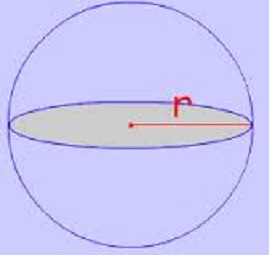
\includegraphics[width=3in]{crosssection_sphere.jpeg}
\end{figure}

To calculate the rate of increase of the area of a cross section we need to calculate
what the radius is at that point.
\begin{align*}
    r = ^3\sqrt{\frac{3V}{4\pi}} = 6in
\end{align*}
Now we just need to differentiate $S_c = \pi r^2$ with respect to time.
\begin{align*}
    \frac{dS_c}{dt} = 2\pi r\frac{dr}{dt} = \frac{6}{25} \pi \: in^2/s \approx 0.754 \: in^2/s
\end{align*}
\textbf{C)} The second bubble is decreasing in volume over time at constant rate of $-3\pi \: in^3/s \approx -9.425 \: in^3/s$.
That means that the radius is also changing. The bubble is smaller smaller and smaller.

\item \textbf{A)} Position is a function of time. To find the velocity we need to 
derive the position equation with respect to time and the acceleration is the $2^{nd}$
derivative of position.
\begin{align*}
    &v(t) = s'(t) = t^2 - 8t + 15\\
    &a(t) = s''(t) = 2t - 8
\end{align*}
\textbf{B)} The time ath which the bug starts walking is t=0. We just need to find s(0).
\begin{align*}
    s(0) = 6
\end{align*}
\textbf{C)} The bug is stopped when v(t) = 0 or when the rate of change of position is 0.
\begin{align*}
    0 &= t^2 - 8t + 15 \\
    0 &= (t-5)\cdot (t-8) \\
    t_1 &= 5 \:|\: t_2 = 8
\end{align*}
\textbf{D)} The bug changes directions when the rate of change of the position is equal to 
zero. If we assume that the bug started to the right than he went left between the first v(t)=0
and the second v(t)=0. Because we have a polynomial function of $3^{rd}$ degree.
We've already solved for v(t)=0. So the bug is going left on the interval $t \in (5; 8)$.
\item \textbf{A)} To find L(x) at x=3 we need to find the slope in that point.
\begin{align*}
    f'(x) = x^2 - 6x \Rightarrow m = -9\\
    \text{Find L(x): } \: L(x) = -9x + 3 
\end{align*}
\textbf{B)} We'll now approximate and also find the real value of f(3.01)
\begin{align*}
    \text{Approximation: }\: L(3.01) = -24.0900\\
    \text{Real value: }\: f(3.01) = -24.0899
\end{align*}
L(3.01) is grater than f(3.01) because it's an overestimation.

\item \textbf{A} We know that r(20) = 3 cm and r'(20)=0.8.
\begin{align*}
    L(t)-3 &= 0.8(t-20) \\
    L(t) &= 0.8t - 13 \Rightarrow L(23) = 5.4 cm
\end{align*}
The linearization value for 23 s is an overestimation because as we can see the
rate of change of the radius is two times less at t=24s than at t=20s

\textbf{B)} We'll just differentiate $V=\frac{4}{3}\pi r^3$ with respect to time.
\begin{align*}
    \frac{dV}{dt} = 4\pi r^2 \frac{dr}{dt} \Rightarrow \frac{dV}{dt|_{t=20}} \approx 90.48\: cm^3/s
\end{align*}
\end{enumerate}



\end{document}